\documentclass[10pt,a4paper,twocolumn]{article}
\RequirePackage[italian]{babel}
\usepackage[utf8]{inputenc}
\usepackage{amsmath}
\usepackage{amsfonts}
\usepackage{amssymb}
\usepackage{graphicx}
\usepackage{sectsty}

\sectionfont{\fontsize{13}{15}\selectfont}
\subsectionfont{\fontsize{11}{12}\selectfont}


\author{M. Faretra, G. Marini, A. Martinelli}
\title{\textbf{Raccolta accurata di fatti da testo in linguaggio naturale di Wikipedia}\\Ricreare Lector utilizzando DBpedia}
\begin{document}
	
\maketitle
\thispagestyle{empty}
\pagestyle{empty}
		
\section*{RIASSUNTO}
		
Molti approcci sono stati tentati nell'ultimo periodo per estrarre informazione da Wikipedia sotto forma di fatti (entità, relazione, entità) per il popolamento di Knowledge Graphs, in particolare sfruttando le informazioni contenute nelle sue \textit{infoboxes}. Tuttavia queste strutture dati riportano solo una piccola parte delle informazioni contenute negli articoli. Infatti nel testo libero si concentra la maggior parte dei fatti estraibili, la rilevazione di essi però risulta più problematica, trovandosi all'interno di un testo in linguaggio naturale, sicuramente più variegato e meno strutturato degli infoboxes. Questi fatti non sono facilmente riconoscibili e dunque estraibili per aumentare la base di conoscenza. 

In questo lavoro propone una metodologia di estrazione di nuovi fatti a partire da questi articoli, con il supporto di un KG già popolato, inoltre si quantifica il numero di nuovi fatti estratti e se ne valuta un campione per verificarne la qualità. In particolare, il nostro lavoro è stato effettuato utilizzando DBpedia, un KG gratuito, che ci ha portato a estrarre circa 1,2 milioni di nuovi fatti, spesso con precisione molto alta.

\section{INTRODUZIONE} 

Le tecniche per l'incremento dei Knowledge Graph in questi ultimi tempi sono state di particolare interesse scientifico e hanno evidenziato la concreta possibilità di aumentare la base di conoscenza che queste strutture possono offrire.

Il progetto DBpedia fornisce informazioni e fatti in 125 linguaggi differenti. La più grande base di conoscenza è estratta dalla versione inglese e consiste in 1,3 miliardi di fatti che descrivono 6 milioni di entità. 

La conoscenza estraibile dal testo libero potrebbe essere decisamente più consistente e aumentare di molto il Knowledge Graph. L'approccio utilizzato va a scalare sfruttando i fatti già contenuti nel KG stesso, è quindi dipendente anche da essi: DBpedia offre una varietà di grafi da poter utilizzare, per questo lavoro sono stati utilizzati due grafi, il primo realizzato a partire dalle informazioni estratte dalle infoboxes fidate, dunque molto pulite; mentre il secondo è stato realizzato a partire sempre dalle infoboxes ma accettando informazioni anche meno pulite rispetto alle prime. I due grafi sono stati utilizzati parallelamente in due processi distinti di estrazione dei fatti.

L'utilizzo di Wikipedia è ampiamente diffuso tra i vari KG esistenti data la grande affidabilità che ormai garantisce, tuttavia le infoboxes fino a pochi anni fa erano ancora molto poco diffuse e solo nell'ultimo decennio esse si trovano in più della metà degli articoli.

Se invece si va a considerare la conoscenza presente nel testo libero, si può immaginare che da esso (ovviamente presente in ogni articolo) si possa estrarre informazione non presente nel KG poiché riporta una serie di informazioni che probabilmente non sono presenti nell'infobox, ad esempio riguardanti anche entità che non sono il soggetto dell'articolo.

Il nostro approccio al problema considera pattern del tipo 
"[entità] frase [entità]", ad esempio: "Ennio Morricone was born in Rome" mette in relazione le due entità \textit{Ennio Morricone} e \textit{Rome} utilizzando la frase "was born in" che descrive, in questo caso, un'istanza della relazione \textit{birthPlace}.

In questo articolo descriviamo l'approccio di estrazione di conoscenza da testo libero di Wikipedia, e i risultati in termini di aumento dei fatti presenti in DBpedia.

Per l'estrazione abbiamo generato dal dump in input, ovvero un insieme di frasi in cui le entità erano già state riconosciute ed etichettate, triple candidate a rappresentare informazione valida, verificando successivamente se la frase della tripla candidata potesse o meno esprimere una relazione. Dopo questa operazione sono state ottenute circa 57 milioni di triple, numero che è stato poi successivamente ridotto di molto, grazie al filtro relazionale fornitoci dal docente.

Il resto dell'articolo è organizzato in vari capitoli: nel Capitolo 2 vengono analizzate in maggior dettaglio le risorse utilizzate; nel Capitolo 3 si presenta l'approccio utilizzato per estrarre nuovi fatti; nel Capitolo 4 vengono mostrati i risultati ottenuti insieme ad alcune analisi puntuali su alcune problematiche riscontrate; nel Capitolo 5 vengono presentate le conclusioni sul lavoro effettuato; nell'ultimo capitolo si discutono alcuni sviluppi futuri che potrebbero rendere il sistema sviluppato più performante.

\section{RISORSE}
\subsection*{\textit{Wikipedia}}

Wikipedia è un'enciclopedia online libera e collaborativa, che attualmente comprende circa 5.3 milioni di articoli nella sua versione inglese. Questa modalità di collaborazione garantisce una grande qualità e affidabilità sulle informazioni ed anche una certa omogeneità nell'esprimere determinati concetti che va a facilitare l'estrazione di fatti utilizzando proprio questi pattern ricorrenti.
 
Ogni articolo in Wikipedia fa riferimento ad una entità principale, che può rappresentare una persona, un luogo, un oggetto, un fatto, ecc..., identificata con un \textit{wiki ID}. Nel testo le informazioni sono codificate in linguaggio naturale, inoltre le entità secondarie eventualmente presenti in un determinato articolo sono rappresentate usando dei \textit{wikilinks}, una sintassi specifica di Wikipedia per evidenziare un particolare concetto e offrire un link all'articolo che lo descrive.

Nel nostro particolare caso le frasi di Wikipedia su cui lavorare ci sono state fornite dal docente già processate dagli strumenti messi a disposizione dall' NLP Group di Stanford, in particolare dallo strumento di Named Entity Recognition, queste erano nella forma di frasi con le entità presenti già etichettate in un particolare formato, ad esempio un frammento di interesse di una frase può essere:

\begin{itemize}
	\item entità soggetto: [[Barack\_Obama$|$m.02mjmr]]
	\item frase: "met"
	\item entità oggetto: [[Donald\_Trump$|$m.0cqt90]]
\end{itemize}

Come si può vedere le entità sono ben identificate e quindi di facile estrazione dalle frasi, inoltre possiedono anche un id che identifica l'entità all'interno di Freebase, non rilevante per questa trattazione.

\subsection*{\textit{DBpedia}}

DBpedia è frutto di un lavoro collaborativo da parte di una moltitudine di utenti per estrarre informazioni da Wikipedia e renderle disponibili sul Web in maniera strutturata.

Ogni entità in DBpedia è identificata da un URI del tipo:
\bigbreak
\textbf{http://dbpedia.org/resource/Name}
\bigbreak
dove \textit{Name} è preso dall'URL del relativo articolo di Wikipedia, che ha la forma:
\bigbreak
\textbf{http://en.wikipedia.org/wiki/Name}.
\bigbreak
In questo modo ogni risorsa è legata direttamente ad un articolo di Wikipedia. I dati sono suddivisi in dataset diversi e dati accessori, in particolare nel nostro caso:

\begin{itemize}
\item dati accessori relativi ai tipi delle entità, ovvero una serie di coppie "URL entità - URL tipo", che associa ad esempio all'entità "Barack Obama" il tipo "OfficeHolder", sottotipo di "Person";

\item dati accessori relativi agli schemi, contenenti informazioni riguardo dominio e codominio di una relazione, oltre a dati sui tipi e supertipi delle entità utilizzati da DBpedia che analizzeremo in seguito;

\item due dataset rappresentanti ognuno un KG, il primo costruito a partire da fonti più affidabili del secondo. Il secondo è stato utilizzato per filtrare i fatti estratti a partire dal primo.
\end{itemize}

\subsection*{\textit{Lector}}

Per estrarre nuovi fatti ed aumentare il grafo è stato seguito un procedimento simile a quello utilizzato originariamente dalla prima versione di Lector, un progetto analogo svolto dal docente e oggetto di studio da parte nostra. Tuttavia si è scelto di variare leggermente alcune fasi del processo estrattivo, oltre che variare anche alcune scelte relativamente allo scoring delle frasi. 
Sebbene il processo estrattivo di Lector si sia rivelato robusto e preciso, lo scopo del nostro progetto è stato anche quello di variare alcuni parametri e alcune modalità di estrazione tanto a scopo esplorativo quanto a scopo sperimentale, includendo anche la possibilità di un peggioramento delle prestazioni rispetto al progetto originale.
Queste modifiche laddove presenti saranno evidenziate nel seguito della trattazione.

\section{APPROCCIO}

Il dataset iniziale di frasi, come detto precedentemente, ci è stato fornito con le entità etichettate. Inizialmente si è provato ad applicare un approccio basato su euristiche per il riconoscimento di frasi di tipo lista, basato sia su il lavoro svolto dal gruppo di NLP di Stanford sia su un lavoro precedentemente svolto da alcuni colleghi. Questo approccio purtroppo si è rivelato non scalabile su una quantità di frasi come quella a disposizione. 

Si è passati poi ad un approccio basato solamente su semplici euristiche, come ad esempio il controllo dei tipi delle entità candidate ad essere quelle nella lista, il controllo molto semplice richiedeva che tutte le entità nella lista fossero dello stesso tipo, oppure la verifica di pattern ricorrenti all'interno di una frase contenente una lista, come il numero di virgole in relazione al numero delle entità, questo è solo un'esempio delle euristiche applicate. Questo approccio si è rivelato efficiente ma non preciso, la quantità di informazione estratta risultava essere poco rilevante rispetto alla mole delle frasi, ulteriori analisi hanno rivelato inoltre che purtroppo questa informazione era quasi sempre non corretta (e.g. l'entità primaria legata alle entità nella lista non erano correlate in nessuna maniera).

\begin{figure}[h]
	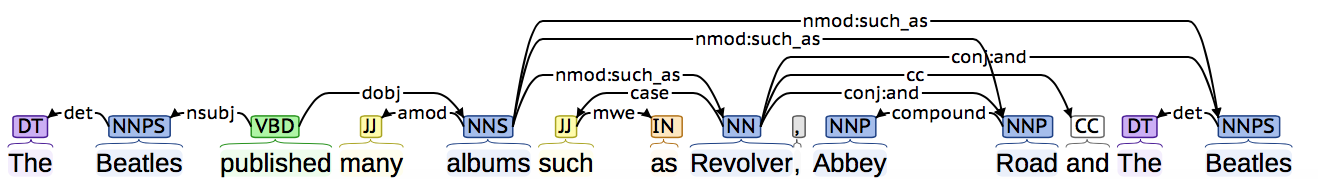
\includegraphics[width=7.7cm, height=1.2cm]{stanford}
	\caption{Esempio di una frase di tipo lista}
\end{figure}

Si è quindi preferito perdere una piccola parte dell'informazione presente nelle frasi favorendo la semplicità, data la grande mole di dati.

Il processamento delle frasi fino ad arrivare all'estrazione dei nuovi fatti si svolge in diversi passaggi:
\begin{enumerate}
\item Pulizia delle frasi originali di Wikipedia, con estrazione di triple entità-frase-entità;
\item Verifica della relazionalità delle frasi che legano due entità;
\item Etichettatura delle triple "presenti" e "non presenti" nel grafo di DBpedia, eseguita due volte, una per ogni grafo;
\item Scoring delle frasi ottenute dal passo precedente;
\item Estrazione dei nuovi fatti, eseguita per entrambi i grafi in modo indipendente.
\end{enumerate}

\subsection{Pulizia delle frasi originali}

Il dump iniziale delle frasi ci è stato fornito dal docente con le entità delimitate da doppie parentesi quadre e arricchite con l'id relativo su \textit{Freebase}, superfluo per questo lavoro. Il dato all'interno di esse ci fornisce il \textit{wiki ID} che è stato utile per reperire l'entità sul grafo di DBpedia, che usa proprio questi identificatori per denotare i nodi. In alcuni casi questi identificatori fanno riferimento ad un \textit{redirect} che punta all'effettivo \textit{wiki ID} reperito tramite una mappatura offerta dal docente, successivamente abbiamo provveduto a sostituire i \textit{redirect} con l'effettivo \textit{wiki ID}.

Abbiamo quindi suddiviso le frasi iniziali in una lista di triple comprendenti tutte le coppie di entità e il testo compreso tra esse, le triple sono state prese in maniera sequenziale, ad esempio se in una frase comparivano 5 entità, le triple sono state estratte nel seguente modo: \textit{ent1-frase1-ent2}, \textit{ent2-frase2-ent3}, ecc.

Le frasi tra le entità sono state quindi passate ad un filtro per trovare quelle relazionali. Quelle che superano il test vengono usate per scremare le triple estratte al passo precedente, prendendo solamente quelle triple che contengono una delle frasi che ha passato il test relazionale. Questa operazione snellisce di molto la quantità di triple estratte garantendo delle triple che quasi sicuramente esprimono una relazione tra due entità.

\subsection{Etichettatura}
A questo punto, abbiamo considerato le coppie di entità di ogni tripla per verificarne l'effettiva presenza all'interno del grafo di DBpedia, sia in quello "fidato" che in quello "non fidato".

Le triple cosiddette "etichettate" rappresentano fatti già presenti nel KG e sono utili per ricavare una mappatura tra le frasi che legano le entità e le relazioni ad esse accomunabili.

Quelle "non etichettate" sono invece candidate a rappresentare quella parte di conoscenza in più che il nostro lavoro tenta di estrarre, ampliando l'informazione presente nel KG.

Le frasi hanno subito una elaborazione molto leggera per ricondurre quelle più particolari a forme più generali in modo da non perdere informazione (e.g.: \textit{was born in} e \textit{was Born in} sono state assimilate alla stessa frase).

\subsection{Scoring}

Ogni frase che lega due entità \textit{"etichettate"} a questo punto è associata ad una o più relazioni definite da DBpedia, ma ovviamente queste corrispondenze potrebbero non rispettare l'effettiva semantica o delle frasi stesse, o della relazione a cui sono associate. Abbiamo quindi assegnato ad ogni frase un punteggio per identificare quelle che secondo lo score definito potrebbero esprimere in maniera corretta la relazione a cui sono collegate, considerando principalmente il numero di volte che esse sono associate con la relazione in esame e il numero di relazioni in cui compare la frase. In questo modo abbiamo cercato di penalizzare frasi che esprimono concetti molto generici, ovvero che compaiono in molte relazioni, poiché non danno molta fiducia sulla correttezza dell'associazione.

Il punteggio viene assegnato tenendo conto del numero di volte che la frase è collegata alla relazione i-esima ( $c(p,r_i)$ ) e del conteggio totale delle sue occorrenze in tutte le relazioni analizzate e trovate nel processo di etichettatura ( $\sum_{j \in R} c(p,r_j)$ ); unendo questi due fattori si ottiene la probabilità originale di Lector:
\[P(r_i|p) = \frac{c(p,r_i)}{\sum_{j \in R}c(p,r_j)}\]
Nel processo di definizione del nuovo score è stato inserito un nuovo fattore moltiplicativo che tiene conto del numero di relazioni a cui è associata la frase in esame ( $c(R|p)$ ).

Il nuovo score risulta essere dunque:
\[score(p,r_i)=c(p,r_i)\cdot P(r_i|p)\cdot \frac{1}{c(R|p)} \]
In questo modo una frase otterrà un punteggio maggiore quanto più compare associata alla relazione in questione rispetto al numero totale di occorrenze, penalizzando inoltre le frasi in base al numero di relazioni a cui sono associate. Questo score penalizza le frasi associate con molte relazioni, tuttavia se la frase è associata con la relazione in esame un numero molto alto di volte allora il primo e il terzo fattore tendono a bilanciarsi, questo è il caso delle frasi che esprimono relazioni ontologiche (e.g. "was a", "is a", ecc...), cioè che sono associate con molte relazioni: il loro "count" per alcune di queste è talmente alto che riescono a ottenere un punteggio molto alto all'interno della relazione in esame.

Un'altra differenza con lo score originale è la rimozione del logaritmo del "count" a favore di un fattore lineare, questo per enfatizzare il ruolo di quest'ultimo nel computo dello score finale. Inoltre non è impostata nessuna soglia sulla probabilità per l'ottenimento delle \textit{top-K} frasi, mentre nell'originale Lector la soglia per permettere ad una frase di far parte delle \textit{top-K} frasi di una relazione era 0.5

\subsection{Estrazione dell'informazione}

\begin{table*}[t]
	\centering
	\label{nuovi-vecchi}
	\begin{tabular}{lllll}
		tipo di grafo utilizzato    & \textit{\#fatti presenti} & \textit{\#nuovi fatti estratti} &  &  \\
		\hline
		grafo con fatti "trusted"   & 14,913,819                & 921,559                         &  &  \\
		grafo con fatti "untrusted" & 11,478,361                & 1,201,154                       &  &  \\
		&                           &                                 &  & 
	\end{tabular}
		\caption{Estrazione dei nuovi fatti in relazione ai fatti già esistenti}
\end{table*}


\begin{table*}[t]
	\centering
	\begin{minipage}{\textwidth}
	
		\begin{tabular}{lllllll}
		\hline \\
		Relazione & \textit{\#"trusted"} & \#n.\textit{"trusted"} & \#n.\textit{"untrusted"} & \#n. comuni & \#eval. & precisione \\
		\hline \\
		birthPlace           & 1,131,887            & 56,554                   & 107,030                    & 56,126       & 100        & 87\%       \\
		deathPlace \footnote{La relazione deathPlace soffre molto del filtraggio, i fatti ottenuti a partire dal grafo "untrusted" non risultano essere imprecisi, tutt'altro, ne risulta dunque una bassissima precisione dovuta al fatto che le triple valutate sono proprio un sottoinsieme sporco dei nuovi fatti "trusted", legati principalmente dalla frase \textit{"moved to"}.}           & 303,537              & 35,392                   & 22,154                     & 17,260       & 100        & 16\%       \\
		nationality          & 123,492              & 3,614                    & 20                         & 0            & 100        & 100\%      \\
		team                 & 778,837              & 9,977                    & 11,520                     & 917          & 100        & 89\%       \\
		almaMater           & 119,573              & 77,944                   & 65,113                     & 63,246       & 100        & 98\%       \\
		spouse               & 35,450               & 6,378                    & 7,081                      & 6,324        & 54         & 50\%       \\
		\hline \\
		parent \footnote{Le relazioni \textit{parent} e \textit{child} hanno dei problemi legati all'omonimia tra gli antenati e i successori, gli strumenti di NER quasi mai riescono a discernere l'antenato dal discendente se questi hanno lo stesso nome, in questi casi abbiamo un fatto in cui soggetto e oggetto puntano entrambi allo stesso \textit{wiki ID} costringendoci a etichettare il fatto come falso.}               & 28,308               & 6,397                    & 8                          & 8            & 100        & 63\%       \\
		child \footnote{Vedi nota \textit{b}.}                & 14,503               & 856                      & 0                          & 0            & 127        & 57,4\%     \\
		ethnicity            & 7,864                & 1,776                    & 1,450                      & 1,303        & 104        & 89,4\%     \\
		religion             & 47,683               & 877                      & 900                        & 596          & 103        & 71,8\%     \\
		award                & 86,279               & 3,087                    & 0                          & 0            & 101        & 94\%       \\
		party                & 81,526               & 3,486                    & 3,614                      & 3,421        & 65         & 95,3\%    
		\end{tabular}
	\end{minipage}
	\caption{Dati relativi alle 12 relazioni di interesse in Lector originale, i fatti valutati sono stati presi eliminando dai nuovi fatti "trusted" i nuovi fatti comuni. \newline Legenda: \textit{\#"trusted"} è il numero di fatti "trusted" già presenti nel corrispondente grafo; \#n.\textit{"trusted"} è il numero di nuovi fatti estratti a partire dal grafo \textit{"trusted"}; \#n.\textit{"untrusted"} è il numero di nuovi fatti estratti a partire dal grafo \textit{"untrusted"}; \#n. comuni è il numero di nuovi fatti comuni ai due insiemi precedenti; \#eval. è il numero di fatti valutati (presi randomicamente all'interno della relazione).}
	\label{dati}
\end{table*}

Una volta ottenuto lo score per ogni frase filtriamo per ogni relazione le 20 frasi (o tutte se ce ne sono meno) con punteggio più alto, queste vengono poi utilizzate per estrarre effettivamente i nuovi fatti. 

A questo punto del procedimento si è reso necessario controllare i tipi delle entità dei fatti candidati a essere estratti. Nello schema fornitoci dal docente le entità note a DBpedia vengono associate ad un tipo, quello più specifico per l'entità (e.g. all'entità Barack\_Obama è associato il tipo \textit{OfficeHolder} il quale però è un sottotipo di \textit{Person}, il quale è un sottotipo di Agent, e così via fino a raggiungere la radice dei tipi \textit{Thing}), le entità dunque sono state arricchite con tutti i loro tipi, si è in pratica scorso l'albero dei tipi dal basso verso l'alto partendo dal tipo associato a ogni entità ottenendo per ogni entità tutti i tipi associati, radice \textit{Thing} inclusa.

Oltre a tipi offerti dalle entità è stato necessario controllare e modificare anche i tipi richiesti dalle relazioni. Molte delle relazioni in DBpedia richiedono che il soggetto e l'oggetto rispettino particolari tipi (e.g la relazione \textit{birthPlace} richiede che il soggetto sia un \textit{Person} mentre l'oggetto sia un \textit{Place}), per ogni relazione si è preso il \textit{domain} della relazione, ovvero il tipo richiesto al soggetto, e il \textit{range}, ovvero il tipo richiesto all'oggetto, e si sono associati alla relazione. Qualora uno dei due non fosse stato definito, il tipo scelto per l'associazione è stato \textit{Thing}. Questa scelta è stata fatta in seguito ad una serie di test, nello schema fornitoci, laddove non ci fosse stato il tipo del \textit{domain} e/o \textit{range}: un'analisi sul portale di DBpedia ha rivelato che il tipo associato al campo mancante era sempre \textit{Thing}, ovvero la radice dei tipi.

Lo stesso discorso è stato applicato per le relazioni che non hanno né \textit{domain} né \textit{range} specificato, che sono: \textit{religion, authority, builder, category, cpu, currency, division, format, gender, hasVariant, honours, influenced, influencedBy, isPartOf, jurisdiction, localAuthority, mainInterest, management, namedAfter, operatedBy, picture, position, predecessor, related, series, similar, source, sportGoverningBody, successor} e \textit{webcast}. Per queste relazioni sia \textit{domain} che \textit{range} sono stati fissati a \textit{Thing}: questa scelta avrebbe potuto portare ad estrarre fatti errati poiché a questo punto non c'è nessuna limitazione sul tipo delle entità legate da una delle suddette relazioni, tuttavia un'analisi svolta sulla relazione \textit{religion} ha dimostrato che la precisione anche senza vincolo dei tipi richiesti risulta essere sufficientemente alta. 

Da notare che grazie al passaggio precedente eseguito sulle entità è possibile che il test del tipo richiesto da una relazione passi, nel caso in cui l'entità su cui si esegue il test offra un sottotipo di quello richiesto (se è offerto \textit{Scientist} e viene richiesto \textit{Person} allora il test passa), ma fallisca nel caso in cui l'entità su cui si esegue il test offra solamente un supertipo di quello richiesto (se è offerto \textit{Person} e viene richiesto \textit{Scientist} il test fallisce), questo è ottenuto senza ulteriori modifiche a \textit{domain} e/o \textit{range} delle relazioni.

Alla luce di quanto detto precedentemente, nella fase di estrazione un nuovo fatto viene estratto se la frase che lega le due entità della tripla è presente nelle \textit{top-K} frasi di una delle relazioni in esame e se i tipi dell'oggetto e del soggetto sono compatibili con quelli richiesti dalla relazione associata alla frase nel passo precedente.  


\section{VALUTAZIONE}

Come possiamo vedere dalla tabella in \ref{nuovi-vecchi} il numero dei nuovi fatti estratti a partire dal grafo considerato meno affidabile è superiore a quello relativo al numero dei nuovi fatti estratti a partire dal grafo più affidabile. Questo è dovuto ad una serie di fattori: ad esempio alcune relazioni del grafo "non fidato" sono assimilabili a una relazione del grafo "fidato", dunque è possibile utilizzare un numero maggiore di \textit{top-K} per estrarre ulteriori fatti.

I 490.503 fatti comuni ai due insiemi di nuovi fatti sono stati utilizzati per filtrare i nuovi fatti estratti a partire dal grafo fidato, ottenendo i nuovi fatti esclusivi dell'estrazione basata sul grafo fidato, il numero di fatti filtrati è dunque 431.056. Per la valutazione successivamente ci siamo concentrati sulle dodici relazioni analizzate originariamente da Lector, ovvero:
\textit{birthPlace, deathPlace, nationality, team, almaMater, spouse, parent, child, ethnicity, religion, award, party} e sul particolare insieme appena definito.

\subsection{\textit{religion}}

In questa sottosezione analizziamo meglio alcuni dei risultati ottenuti riguardanti le relazioni che non offrono né \textit{domain} e né \textit{range} all'interno dello schema di DBpedia. Prendiamo la relazione \textit{religion} come esempio, questa non definisce né dominio né codominio, come detto prima la nostra scelta è stata quella di considerare corretto il tipo di qualsiasi entità associata a questo insieme di relazioni.

Questa scelta porta ad estrarre fatti molto eterogenei tra loro, in particolare gli errori riscontrati si sono visti in caso di entità associate mediante le frasi \textit{practice, practices}, queste possono essere sicuramente collegate al dominio religioso, ma molto più spesso si riconducono al dominio sportivo. Una scelta più accurata dei tipi delle entità che possono essere legate da questo insieme di relazioni potrebbe aumentare la precisione di molti punti percentuali, portandola quasi ai valori di Lector.

\subsection{\textit{child} e \textit{parent}}\label{child&parent}

Queste due relazioni sono di difficile gestione, la precisione risulta essere più bassa dell'originale Lector, tuttavia questo è dovuto non alla presenza di frasi fuorvianti come ad esempio \textit{was succeeded by}, frase che nelle originali estrazioni portava dei fatti non corretti. 

In questo caso, in quasi la totalità dei fatti etichettati come non corretti, sono presenti casi di omonimia tra successore/discendente, ad esempio \textit{John Christopher Smith jr.} è il figlio di \textit{John Christopher Smith}, gli strumenti di NER spesso non sono riusciti a comprendere quale sia il \textit{wiki ID} del figlio e quale il \textit{wiki ID} del padre, sostanzialmente i due non sono assolutamente distinti e il risultato è che il fatto riporta lo stesso \textit{wiki ID} sia per il soggetto che per l'oggetto.

Questi fatti dunque risultano collegare due entità identiche, come se il figlio fosse padre di se stesso e viceversa, costringendoci ad etichettare il fatto come falso. Se si isolano questi fatti da quelli valutati il rimanente insieme dei fatti assume una precisione molto vicina al 100\%.

\subsection{\textit{deathPlace}} \label{deathPlace}

La relazione \textit{deathPlace} è quella con la precisione più bassa, tuttavia analizzarla ci ha permesso di comprendere alcuni fattori importanti: come è possibile vedere dalla tabella il numero di fatti nuovi a partire dal grafo "trusted" è a volte simile se non inferiore al numero di nuovi fatti "untrusted". Per come è stata fatta l'analisi dei nuovi fatti, quelli valutati sono un sottoinsieme esclusivo dei fatti "trusted", ma analizzando anche quelli "untrusted" si è visto che questi tendono ad avere una precisione molto più alta, almeno nel caso della relazione in esame.

Questa discordanza di precisione tra i fatti dei due insiemi ci porta a dire che per alcune relazioni è possibile che i fatti estratti possano avere precisione simile qualunque sia il grafo di partenza utilizzato: potrebbe essere dunque utile unire i due grafi di partenza in modo tale da non creare problemi legati alla precisione nella fase di estrazione riguardante questo tipo di relazioni, qualora questa venga effettuata con il filtraggio dei fatti come è stata eseguita nel nostro lavoro.

\section{CONCLUSIONI}

In questa trattazione è stato illustrato il processo di estrazione che ci ha portato a identificare più di un milione di nuovi fatti non presenti in DBpedia, inoltre sono state analizzate a fondo alcune relazioni importanti nel dominio delle persone. \'E stato visto come è possibile estrarre una buona quantità di nuovi fatti con una precisione che può arrivare ad essere prossima al 100\%. 

Inoltre è stato visto come in alcuni casi laddove la precisione risulta essere molto più bassa di quanto ci si può aspettare, i problemi possono essere legati ai sistemi di preprocessamento del testo quali ad esempi gli strumenti di NER, e che tolti quei fatti affetti da questi problemi la precisione sale di molti punti percentuali fino ad arrivare a valori molto prossimi al 95-100\%, questo a riprova che il metodo di estrazione è sufficientemente robusto e preciso.

\section{SVILUPPI FUTURI}

In un futuro si potrebbero svolgere varie attività utili al miglioramento del processo di estrazione, alcune di queste possono riguardare la definizione di \textit{domain} e \textit{range} per quelle relazioni che non lo prevedono nello schema. Questo potrebbe portare ad un ulteriore filtraggio dei fatti, lasciando passare solo quelli che rispettano il nuovo vincolo relazionale, probabilmente aumentando di conseguenza la precisione ai valori dell'originale Lector.\footnote{Vedi Tabella \ref{dati}}

Un'altra attività che si può svolgere è l'unione dei due dataset iniziali, ovvero del grafo "trusted" e del grafo "untrusted", nella fase di estrazione e di valutazione: è stato visto che i fatti nel grafo "untrusted" sono sicuramente di qualità inferiore ma non così inferiori come si è pensato quando sono stati svolti i primi passi nella realizzazione del sistema. Questo potrebbe portare ad un aumento del numero dei nuovi fatti, al costo di un abbassamento della precisione di questi ultimi che potrebbe risultare irrisorio, in alcuni casi quindi questa unione può essere vantaggiosa.\footnote{Vedi \ref{deathPlace}}

Un'ultima riflessione che è possibile fare riguarda l'eterogeneità delle relazioni presenti nel grafo "untrusted": questo infatti ospita una moltitudine di relazioni o \textit{properties}, che si possono spesso riunire in gruppi di 2-3 elementi ed assimilare ad una relazione particolare delle relazioni "trusted"; ad esempio le \textit{properties} \textit{placeOfBirth} e \textit{birthPlace} possono essere assimilate entrambe alla stessa relazione "trusted", ovvero \textit{ontology/birthPlace}. L'assimilazione permetterebbe di ottenere più fatti "untrusted" nuovi per singola relazione, cosa che permette di filtrare con maggiore qualità i nuovi fatti "trusted". Tuttavia come abbiamo illustrato prima questo filtraggio può anche portare ad un abbassamento drastico della precisione dei nuovi fatti, come visto ad esempio nella relazione \textit{deathPlace}.

\end{document}